\documentclass[../main]{subfiles}

\begin{document}

\clearpage

\setcounter{eqnarray}{0}
\setcounter{equation}{0}
\setcounter{figure}{0}

\part*{第4回}

\subsection{ベクトル場の回転とのStokesの定理}
\subsubsection{線積分}
例を通じて{\bf 線積分}を学ぶ.\\

{\bf 例1}\\
物体が力Fを受けて直線上をl動いたとき,力Fがした仕事は$F \times l$ \\

{\bf 例2}\\
力{\bf F}がした仕事は,変位を表すベクトルを${\bf l}$,なす角を$\theta$とすると,
${\bf F} \cdot {\bf l}=Fl \cos \theta$ \\

{\bf 例3}\\
\begin{figure}[htbp]
 \begin{center}
  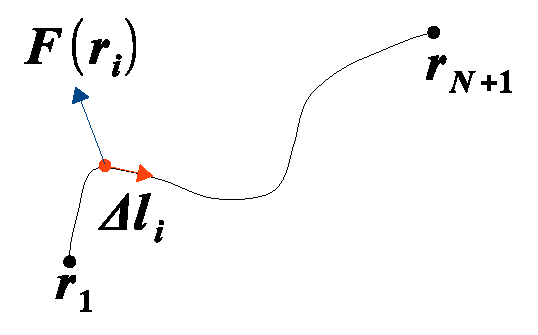
\includegraphics[width=80mm]{4.1.eps}
 \end{center}
 \caption{}
 \label{fig:one}
\end{figure}
物体が力{\bf F}を受けて,経路上を,移動するとき,\\
まず経路をN区間に分割する.分割点それぞれの位置が${\bf r}_i$,経路の始点と終点の位置が${\bf r}_1$,${\bf r}_{N+1}$であるとすると, \\
分割が十分細かければ,物体は各区間では,${\bf r}_i$から${\bf r}_{i+1}$に向かうベクトル${\bf \Delta l}_i$の方向に運動し,力が一定と見なせる.
したがって各区間で力{\bf F}が物体にした仕事は,${\bf F}({\bf r}_i) \cdot {\bf \Delta l}_i$となる.
これを全区間にわたって足し合わせて,分割を十分細かくする($N \to \infty$)と,変位ベクトルの長さ$|{\bf \Delta l}_i|$は0に近づき,Fがした仕事について以下の式が得られる.

\begin{equation}
\int_{C}^{} {\bf F} \cdot {\bf dl} = \lim_{|{\bf \Delta l}_i| \to 0, N \to \infty} \sum_{i=1}^{N} {\bf F}({\bf r}_i) \cdot {\bf \Delta l}_i
\end{equation}
ここでCとは向きがある経路({\bf 有向経路})である.\\

簡単な場合について考える.\\
C上で常に,
\begin{equation}
\left \{
\begin{array}{l}
{\bf \Delta l}_i // {\bf F}({\bf r}_i) \\
\mbox{力の大きさ}|{\bf F}({\bf r}_i)|\mbox{がiによらず一定}
\end{array}
\right.
\end{equation}
が成り立つ場合,
\begin{equation}
\int_{C}^{} {\bf F} \cdot {\bf dl} = F \times \mbox{(有向経路Cの長さ)} \times (\pm 1)
\end{equation}
ただし,$\pm 1$は運動の向きによる.\\

\subsubsection{ベクトル場の回転}
ベクトル場{\bf A}の渦巻き具合を定式化する.
まず閉じた有向経路({\bf 有向ループ})について,{\bf 渦}を以下のように定義する.
\begin{itembox}[c]{有向ループCについてのベクトル場{\bf A}の{\bf 渦(vortex)}}
\begin{equation}
\int_{C}^{} {\bf A} \cdot {\bf dl}
\end{equation}
\end{itembox}
空間の1点での渦を定式化したい.\\
\begin{figure}[htbp]
 \begin{center}
  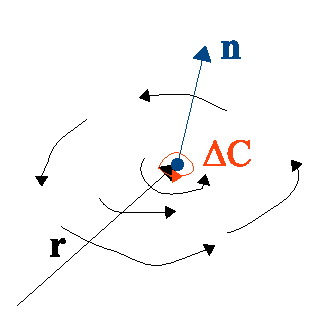
\includegraphics[width=50mm]{4.2.eps}
 \end{center}
 \caption{}
 \label{fig:two}
\end{figure}
そのために単位面積あたりの渦について考えてから,有向ループを小さくしていく.\\
微小有向ループがある平面上にあるとすると,平面に対する法線ベクトル{\bf n}をとることができる.\\
ただし{\bf n}と垂直な平面内の微小有向ループ$\Delta C$に沿って右ねじを巻いたとき,ねじが+{\bf n}方向に進み,{\bf n}は単位ベクトルとする.
単位面積あたりの渦は,渦を微小有向ループの囲む面積で割ると得られる.
\begin{equation}
\frac{\int_{C}^{} {\bf A} \cdot {\bf dl}}{\mbox{($\Delta C$の囲む面積)}}
\end{equation}
微小ループを小さくした極限を,ベクトル場{\bf A}の,位置{\bf r}における{\bf 回転(rotation)}といい,{\rm rot}{\bf A}と表す.これは大きさが式(5)で表せ,方向が微小有向ループのある平面の法線と等しいベクトルである.
\begin{itembox}[c]{ベクトル場{\bf A}の位置{\bf r}における回転の{\bf n}方向成分}
\begin{equation}
({\rm rot}{\bf A})_{\bf n} =\lim_{\Delta C \to 0}  \frac{\int_{C}^{} {\bf A} \cdot {\bf dl}}{\mbox{($\Delta C$の囲む面積)}}
\end{equation}
\end{itembox}
ベクトル場の{\bf 回転}には以下の式が成り立つ.
\begin{equation}
\mathrm{rot}{\bf A} =
\left( 
\begin{array}{cc}
\frac{\partial A_z}{\partial y}-\frac{\partial A_y}{\partial z}\\
\\
\frac{\partial A_x}{\partial z}-\frac{\partial A_z}{\partial x}\\
\\
\frac{\partial A_y}{\partial x}-\frac{\partial A_x}{\partial y}\\
\end{array}
\right)
\end{equation}
{\bf 証明} \\
回転のz成分$(\mathrm{rot}{\bf A})_z$ のみ導出する.\\
\begin{figure}[htbp]
 \begin{center}
  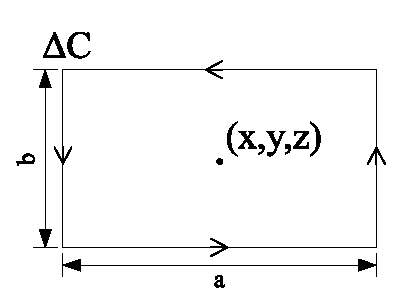
\includegraphics[width=80mm]{4.3.eps}
 \end{center}
 \caption{}
 \label{fig:three}
\end{figure}
\\
\begin{center}
\bf{有向ループに垂直な単位ベクトル{\bf n}:z軸方向} \\
\bf{ $\Delta C$:xy平面内の\uwave{微小}ループ} \\
\end{center}
\begin{eqnarray}
\int_{C}^{} {\bf A} \cdot {\bf dl} &=& a( A_x(x,y-\frac{b}{2},z)-A_x(x,y+\frac{b}{2},z) ) \\
&+&b ( A_y(x+\frac{a}{2},y,z)-A_y(x-\frac{a}{2},y,z) )
\end{eqnarray}
1.7節の証明で用いたのと同様の近似によって,
\begin{eqnarray}
A_x(x,y-\frac{b}{2},z) = A_x(x,y,z)-\frac{b}{2} \frac{\partial A_x}{\partial y} \\
A_x(x,y+\frac{b}{2},z) = A_x(x,y,z)+\frac{b}{2} \frac{\partial A_x}{\partial y}
\end{eqnarray}
差をとって
\begin{eqnarray}
A_x(x,y-\frac{b}{2},z)-A_x(x,y+\frac{b}{2},z) = -b \frac{\partial A_x}{\partial y}
\end{eqnarray}
同様に
\begin{eqnarray}
A_y(x+\frac{a}{2},y,z)-A_y(x-\frac{a}{2},y,z) = a \frac{\partial A_y}{\partial y}
\end{eqnarray}
したがって$a,b \to 0$ においては
\begin{eqnarray}
\int_{C}^{} {\bf A} \cdot {\bf dl} \to ab \left( \frac{\partial A_y}{\partial x} - \frac{\partial A_x}{\partial y} \right)
\end{eqnarray}
よって
\begin{eqnarray}
({\rm rot} {\bf A})_z = \lim_{a,b \to 0} \frac{1}{ab} \int_{C}^{} {\bf A} \cdot {\bf dl} =\frac{\partial A_y}{\partial x} - \frac{\partial A_x}{\partial y}
\end{eqnarray}
$({\rm rot} {\bf A})_x$ , $({\rm rot} {\bf A})_y$ も同様に導かれる.
\begin{flushright}
(証明終)
\end{flushright}

{\bf 例} \\
${\bf A} = (-ky,kx,0)$,$k>0$ つまり,平面一様に渦がある場合.\footnote{渦の様子を描いてみると良いでしょう.} 
\begin{eqnarray}
{\rm rot}{\bf A} =  
\left( 
\begin{array}{cc}
\frac{\partial A_z}{\partial y}-\frac{\partial A_y}{\partial z}\\
\\
\frac{\partial A_x}{\partial z}-\frac{\partial A_z}{\partial x}\\
\\
\frac{\partial A_y}{\partial x}-\frac{\partial A_x}{\partial y}\\
\end{array}
\right)
=
\left( 
\begin{array}{cc}
\frac{\partial}{\partial y}(0)-\frac{\partial}{\partial z}(kx)\\
\\
\frac{\partial}{\partial z}(-ky)-\frac{\partial}{\partial x}(0)\\
\\
\frac{\partial}{\partial x}(kx)-\frac{\partial}{\partial y}(-ky)\\
\end{array}
\right)
=
\left( 
\begin{array}{cc}
0 \\
\\
0 \\
\\
2k \\
\end{array}
\right)
\end{eqnarray}
\\
ベクトル場の回転は線形性を有する.
\begin{equation}
\left \{
\begin{array}{l}
{\rm rot}(\alpha {\bf A}) = \alpha {\rm rot}{\bf A} \\
{\rm rot}({\bf A}+{\bf B}) = {\rm rot}{\bf A} + {\rm rot}{\bf B}
\end{array}
\right.
\end{equation}

\subsubsection{Stokesの定理}
\begin{figure}[htbp]
 \begin{center}
  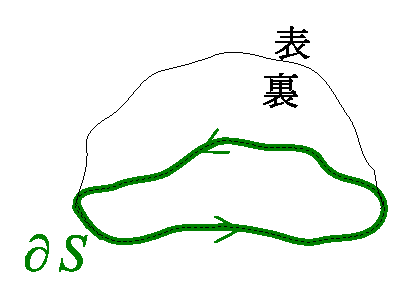
\includegraphics[width=80mm]{4.4.eps}
 \end{center}
 \caption{}
 \label{fig:four}
\end{figure}
表裏つき曲面Sについて$\partial S$をSの境界として定まる有向ループとする.\footnote{分かり難くて申し訳ありませんが,この図の場合はヘルメットのような曲面を想定しています.} \\
$\partial S$の方向は,それに沿って右ねじを巻くとSを裏から表に貫くように定める.
すると以下の定理が成り立つ.
\begin{itembox}[c]{Stokesの定理}
\begin{eqnarray}
\int_{\partial S}^{} {\bf A} \cdot {\bf dl} = \int_{S}^{} {\rm rot}{\bf A} \cdot {\bf dS} \\
\mbox{ふちに沿った線積分} = \mbox{回転の面積分}
\end{eqnarray}
\end{itembox}
{\bf 証明} \\
\begin{figure}[htbp]
 \begin{center}
  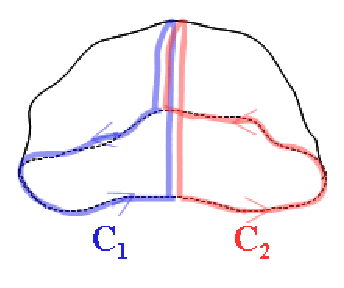
\includegraphics[width=80mm]{4.5.eps}
 \end{center}
 \caption{}
 \label{fig:five}
\end{figure}
曲面を曲面上の曲線によって2つに分割すると,曲面の境界として定まる有向ループも2つになる.2つの有向ループは共通部分をもつが,その方向は逆となっているのでその部分の線積分は打ち消しあい,分割前の線積分と等しくなる.\\
したがって分割を繰り返しても有向ループに沿ったベクトル場の線積分は不変であるので,
\begin{eqnarray}
\int_{\partial S}^{} {\bf A} \cdot {\bf dl} &=& \int_{C_1}^{} {\bf A} \cdot {\bf dl} + \int_{C_2}^{} {\bf A} \cdot {\bf dl} \\
&=& \sum_{i=1}^{N} \int_{C_i}^{}{\bf A} \cdot {\bf dl} \\
&=& \sum_{i=1}^{N} \mbox{($C_i$の囲む面積)}\frac{1}{\mbox{($C_i$の囲む面積)}}\int_{C_i}^{}{\bf A} \cdot {\bf dl}
\end{eqnarray}
ここで
\begin{eqnarray}
({\rm rot}{\bf A})_{n_i} = \frac{1}{\mbox{($C_i$の囲む面積)}}\int_{C_i}^{}{\bf A} \cdot {\bf dl}
\end{eqnarray}
である.また,$C_i$の囲む面積を$\Delta S_i$ とすると, $N \to \infty$において次々に
\begin{eqnarray}
\int_{\partial S}^{} {\bf A} \cdot {\bf dl} &\to& \sum_{i} \Delta S_i ({\rm rot}{\bf A})_{n_i} \\
&\to& \int_{S}^{} {\rm rot}{\bf A} \cdot {\bf dS}
\end{eqnarray}
\begin{flushright}
(証明終)
\end{flushright}
{\bf 例} \\
\begin{eqnarray}
{\bf A} =  
\left( 
\begin{array}{cc}
-ky \\
\\
kx \\
\\
0 \\
\end{array}
\right)
,
{\rm rot}{\bf A} =  
\left( 
\begin{array}{cc}
0 \\
\\
0 \\
\\
2k
\end{array}
\right)
\end{eqnarray}
であるとき,
\begin{eqnarray}
\int_{\partial S}^{} {\bf A} \cdot {\bf dl} = kr \times 2 \pi r = 2 \pi k r^2 \\
\int_{S}^{} {\rm rot}{\bf A} \cdot {\bf dS} = 2k \times \pi r^2  = 2 \pi k r^2
\end{eqnarray}
\subsubsection{まとめ}
\begin{eqnarray}
\int_{S}^{} {\bf A} \cdot {\bf dS} \mbox{(湧き出し)} \xrightarrow[]{\mbox{単位体積あたり,極限}} {\rm div}{\bf A}\mbox{(発散)} : \mbox{スカラー} : \mbox{Gaussの定理} \\
\int_{C}^{}{\bf A} \cdot {\bf dl} \mbox{(渦)} \xrightarrow[]{\mbox{単位面積あたり,極限}} {\rm rot}{\bf A}\mbox{(回転)} : \mbox{ベクトル} : \mbox{Stokesの定理}
\end{eqnarray}

\end{document}
